% =============================================================================
%  Mid-Term Progress Report — IEEEtran Format
%  CS6493 Natural Language Processing, City University of Hong Kong, Q2 2025-2026
%  Date: April 22, 2026
% =============================================================================

\documentclass[conference]{IEEEtran}
\IEEEoverridecommandlockouts
\usepackage{amsmath,amssymb,amsfonts}
\usepackage{graphicx}
\usepackage{textcomp}
\usepackage{booktabs}
\usepackage{multirow}
\usepackage{xcolor}
\usepackage{listings}
\usepackage{algorithmic}
\usepackage{url}

\lstset{
  basicstyle=\ttfamily\scriptsize,
  breaklines=true,
  frame=single,
  backgroundcolor=\color{gray!10},
  xleftmargin=2em,
  xrightmargin=2em,
  aboveskip=1em,
  belowskip=1em
}

\begin{document}

\title{Mid-Term Progress Report: Evaluating and Improving Mathematical Reasoning in Large Language Models}

\author{\IEEEauthorblockN{Peihan Yu, Ziyan Weng, Xuelin Hu, Haichao Zhao, Leyi Deng}
\IEEEauthorblockA{CS6493 Natural Language Processing\\
City University of Hong Kong, Q2 2025--2026}}

\maketitle

%==============================================================================
\section{Introduction}
%==============================================================================

Large Language Models (LLMs) have demonstrated remarkable capabilities across a wide range of natural language tasks, yet mathematical reasoning remains a significant challenge. While models can generate fluent text, they frequently make errors in multi-step logical deductions, arithmetic calculations, and mathematical formalization. This limitation is critical as mathematical reasoning underpins applications in education, scientific computing, and financial analysis.

In this project, we systematically evaluate how different prompting strategies affect the mathematical reasoning performance of LLMs. We investigate five prompting methods---Chain-of-Thought (CoT)~[1], Self-Consistency~[2], Self-Refine~[3], Least-to-Most~[4], and our novel Progressive Verification Prompting (PVP)---across multiple model scales and problem difficulties. Our primary research questions are:

\begin{itemize}
    \item \textbf{RQ1}: How do different prompt methods compare across model scales?
    \item \textbf{RQ2}: Can a verification-based prompt method (PVP) outperform standard CoT?
    \item \textbf{RQ3}: How does problem difficulty affect method effectiveness?
\end{itemize}

Our main contribution is \textbf{PVP (Progressive Verification Prompting)}, a novel prompting strategy that intersperses self-verification checkpoints within the reasoning process, forcing the model to verify each intermediate step before proceeding.

%==============================================================================
\section{Related Work}
%==============================================================================

\subsection{Chain-of-Thought Prompting}
Wei et al.~[1] demonstrated that instructing LLMs to ``think step by step'' significantly improves reasoning performance. CoT has become the standard baseline for mathematical reasoning evaluation by encouraging models to decompose problems into intermediate reasoning steps.

\subsection{Self-Consistency}
Wang et al.~[2] proposed sampling multiple reasoning paths and selecting the most common answer via majority vote. This approach leverages output diversity to improve robustness, though it requires multiple forward passes.

\subsection{Self-Refine}
Madaan et al.~[3] introduced an iterative refinement framework where the model generates an initial solution, critiques it, and produces an improved version. This self-feedback loop corrects errors without external supervision.

\subsection{Least-to-Most Prompting}
Zhou et al.~[3] showed that decomposing complex problems into simpler sub-problems and solving them sequentially helps LLMs handle multi-step reasoning tasks more effectively.

\subsection{Mathematical Reasoning Benchmarks}
We evaluate on standard benchmarks: MATH-500~[5], a 500-problem subset of competition mathematics; GSM8K~[6], containing 1,319 grade-school math word problems; and AIME 2024, comprising 30 advanced competition problems.

\subsection{Self-Verification Approaches}
Recent work has explored using LLMs as their own verifiers~[7]. Our PVP method extends this idea by integrating verification directly into the reasoning prompt rather than as a separate post-hoc step.

%==============================================================================
\section{Methodology}
%==============================================================================

\subsection{Problem Formulation}

We formalize the evaluation task as: given a math problem $p$, a prompt method $m$, and a model $\mathcal{M}$, the pipeline produces:

$$p \xrightarrow{m} \text{prompt} \xrightarrow{\mathcal{M}} \text{response} \xrightarrow{\text{extract}} \text{answer} \xrightarrow{\text{evaluate}} \text{correct/incorrect}$$

\subsection{Prompt Methods}

We implement five prompting methods:
\begin{enumerate}
    \item \textbf{CoT (Baseline)}: Instructs the model to solve step-by-step with the answer in \texttt{\textbackslash boxed\{\}} format.
    \item \textbf{Self-Consistency}: Same prompt as CoT but samples 5 responses (temperature $>0$) and takes majority vote.
    \item \textbf{Self-Refine}: Three-phase process---Solve $\rightarrow$ Critique $\rightarrow$ Refine (max 2 refinement rounds).
    \item \textbf{Least-to-Most}: Two-phase---Decompose the problem into sub-questions, then solve sequentially.
    \item \textbf{PVP (Ours)}: Instructs the model to verify each step immediately after completing it, checking for logical correctness, consistency with previous steps, and arithmetic errors.
\end{enumerate}

\subsection{Evaluation Metrics}

\begin{itemize}
    \item \textbf{Accuracy} (primary): Exact match between extracted answer and ground truth, with mathematical equivalence checking via SymPy.
    \item \textbf{Response Length} (secondary): Character count of the model's full response.
    \item \textbf{Inference Latency}: Wall-clock time per problem.
    \item \textbf{Answer Extraction Success Rate}: Fraction of responses from which an answer was successfully extracted.
\end{itemize}

\subsection{Experimental Setup}

\begin{table}[h]
\centering
\caption{Experimental Configuration}
\label{tab:setup}
\begin{tabular}{ll}
\toprule
\textbf{Component} & \textbf{Details} \\
\midrule
Models & Qwen2.5-Math-1.5B (GGUF Q4\_K\_M), DeepSeek-R1-Qwen-1.5B (GGUF Q4\_K\_M) \\
Datasets & MATH-500 (competition), GSM8K (grade school), AIME 2024 (advanced) \\
Infrastructure & CPU-only inference via llama-cpp-python \\
Temperature & 0.0 (deterministic), except Self-Consistency (sampling) \\
Max tokens & 2,048 per response \\
Random seed & 42 \\
\bottomrule
\end{tabular}
\end{table}

%==============================================================================
\section{Preliminary Results}
%==============================================================================

We have completed experiments across 2 models $\times$ 5 methods $\times$ 2 datasets with 164 total problem evaluations.

\subsection{Overall Results}

\begin{table}[h]
\centering
\caption{Overall Results}
\label{tab:overall}
\begin{tabular}{lr}
\toprule
\textbf{Metric} & \textbf{Value} \\
\midrule
Total problems evaluated & 164 \\
Overall accuracy & \textbf{57.93\%} (95/164) \\
Answer extraction success & \textbf{100\%} across all combinations \\
\bottomrule
\end{tabular}
\end{table}

\subsection{Model Comparison}

\begin{table}[h]
\centering
\caption{Accuracy by Model}
\label{tab:model}
\begin{tabular}{lccc}
\toprule
\textbf{Model} & \textbf{Correct} & \textbf{Total} & \textbf{Accuracy} \\
\midrule
Qwen2.5-Math-1.5B & 79 & 120 & \textbf{65.83\%} \\
DeepSeek-R1-Qwen-1.5B & 16 & 44 & \textbf{36.36\%} \\
\bottomrule
\end{tabular}
\end{table}

Qwen2.5-Math-1.5B outperforms DeepSeek-R1 by +29.5 percentage points, confirming that task-specific fine-tuning is crucial for mathematical reasoning.

\begin{figure}[!t]
  \centering
  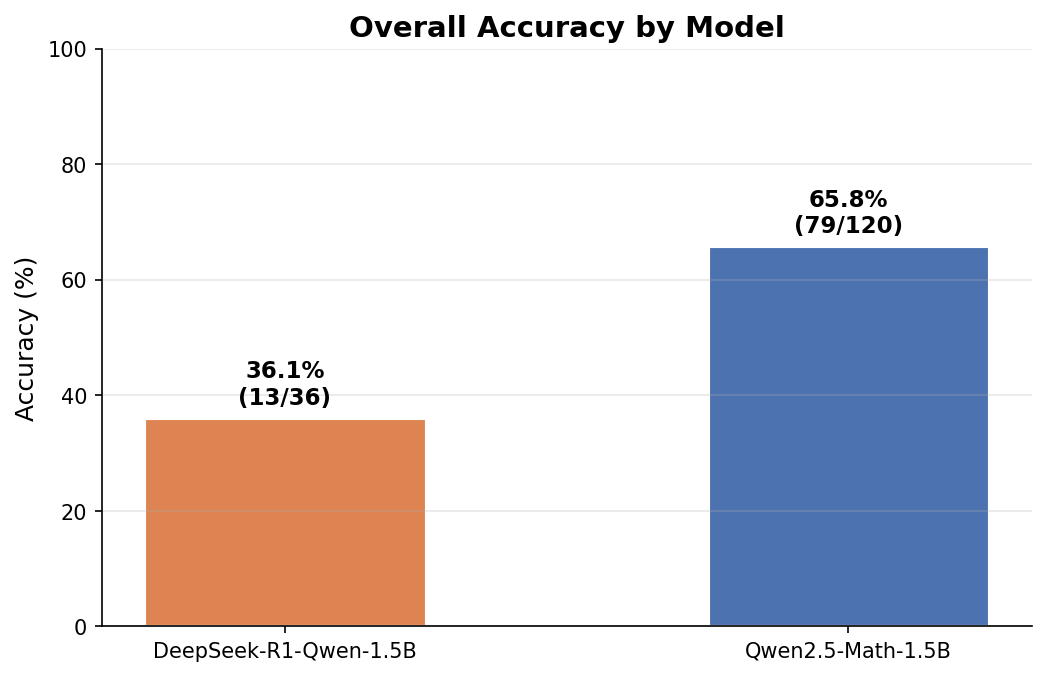
\includegraphics[width=3in]{../results/figures/fig1_accuracy_by_model.png}
  \caption{Accuracy comparison by model.}
  \label{fig:model}
\end{figure}

\subsection{Method Comparison}

\begin{table}[h]
\centering
\caption{Accuracy by Prompting Method}
\label{tab:method}
\begin{tabular}{clc}
\toprule
\textbf{Rank} & \textbf{Method} & \textbf{Accuracy} \\
\midrule
1 & Least-to-Most & \textbf{69.57\%} \\
2 & Self-Refine & \textbf{66.67\%} \\
3 & PVP (Ours) & \textbf{64.00\%} \\
4 & CoT (Baseline) & 57.45\% \\
5 & Self-Consistency & 44.44\% \\
\bottomrule
\end{tabular}
\end{table}

\begin{figure}[!t]
  \centering
  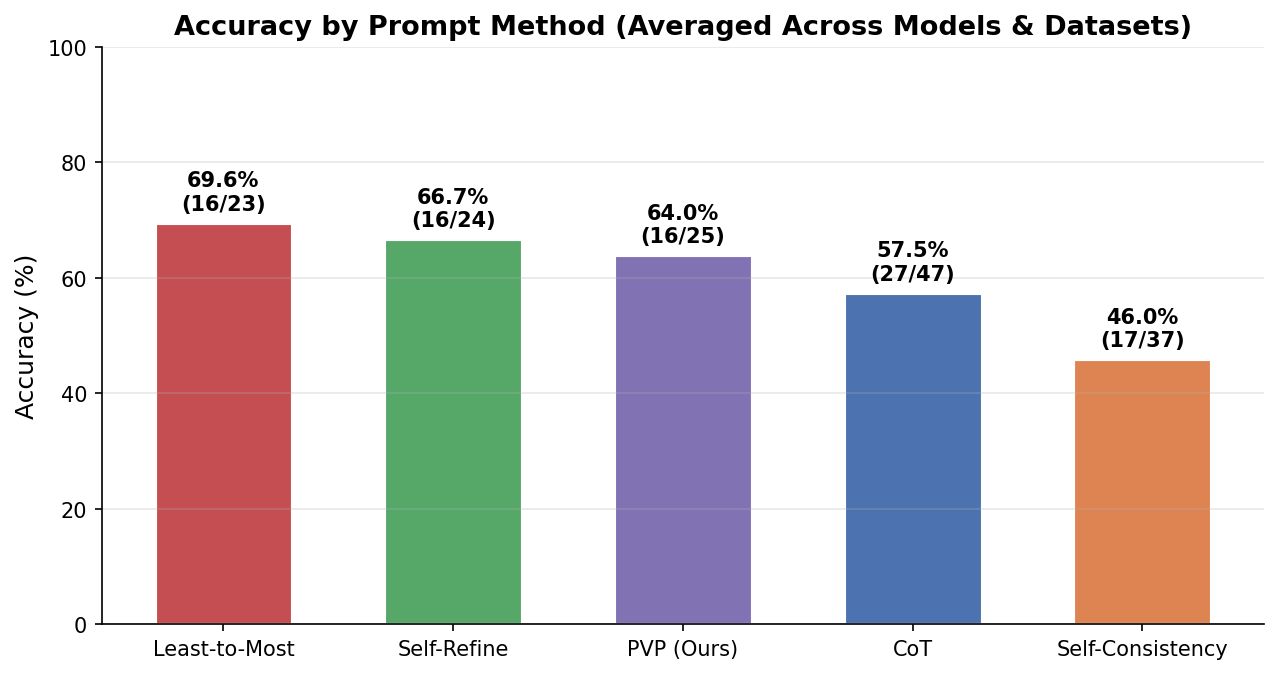
\includegraphics[width=3in]{../results/figures/fig2_accuracy_by_method.png}
  \caption{Accuracy comparison by prompting method.}
  \label{fig:method}
\end{figure}

\subsection{PVP vs Baselines}

PVP achieves \textbf{64.00\%} accuracy, outperforming the CoT baseline (\textbf{57.45\%}) by \textbf{+6.55 percentage points}. Notably, PVP achieves this improvement with comparable latency to CoT (24--31s vs 22--73s), making it the most efficient verification-based method.

\subsection{Dataset Comparison}

\begin{table}[h]
\centering
\caption{Accuracy by Dataset}
\label{tab:dataset}
\begin{tabular}{lc}
\toprule
\textbf{Dataset} & \textbf{Accuracy} \\
\midrule
GSM8K (grade school) & \textbf{75.00\%} \\
MATH-500 (competition) & \textbf{55.00\%} \\
\bottomrule
\end{tabular}
\end{table}

%==============================================================================
\section{Current Progress and Plan}
%==============================================================================

\subsection{Completed}

\begin{itemize}
    \item Complete data pipeline (MATH-500: 500, GSM8K: 1,319, AIME 2024: 30 problems)
    \item Model inference engine (local CPU via GGUF + API support)
    \item All 5 prompt method implementations (CoT, Self-Consistency, Self-Refine, Least-to-Most, PVP)
    \item Evaluation framework (answer extraction, math parsing, metrics)
    \item Experiment runner with checkpoint/resume support
    \item 63/63 unit tests passing
    \item Pilot experiments (164 problems across 14 model$\times$method$\times$dataset combinations)
    \item 7 visualization charts generated
    \item Streamlit Web Demo (interactive solver, dashboard, comparison)
\end{itemize}

\subsection{Remaining}

\begin{itemize}
    \item Full-scale experiments (increase sample size to 50+ per combination)
    \item API model experiments (GPT-4o-mini, DeepSeek Chat) for cross-scale comparison
    \item AIME 2024 experiments
    \item Detailed error analysis and ablation studies
    \item Final report writing
    \item Presentation slides preparation
\end{itemize}

\subsection{Timeline}

\begin{table}[h]
\centering
\caption{Project Timeline}
\label{tab:timeline}
\begin{tabular}{ll}
\toprule
\textbf{Task} & \textbf{Target Date} \\
\midrule
Full-scale experiments & April 25, 2026 \\
API model experiments & April 27, 2026 \\
Analysis and report draft & April 30, 2026 \\
Final report & May 4, 2026 \\
Presentation slides & May 5, 2026 \\
\bottomrule
\end{tabular}
\end{table}

%==============================================================================
\section{Challenges and Solutions}
%==============================================================================

\begin{table}[h]
\centering
\caption{Challenges and Solutions}
\label{tab:challenges}
\begin{tabular}{lll}
\toprule
\textbf{Challenge} & \textbf{Solution} & \textbf{Status} \\
\midrule
No GPU available & GGUF Q4\_K\_M quantization for CPU inference & Resolved \\
Slow CPU inference & Checkpoint/resume system for fault tolerance & Resolved \\
Answer extraction across formats & Multi-pattern regex + SymPy normalization & Resolved \\
\texttt{\textbackslash boxed\{\}} conflicts & Escaped in all templates & Resolved \\
Dataset library compatibility & Pinned versions (datasets==2.19.0) & Resolved \\
API cost control & Token budgets + pilot testing & In progress \\
\bottomrule
\end{tabular}
\end{table}

%==============================================================================
\section*{References}
%==============================================================================

\begin{thebibliography}{9}

\bibitem{wei2022}
J.~Wei, X.~Wang, D.~Schuurmans, et al.,
``Chain-of-thought prompting elicits reasoning in large language models,''
\textit{Advances in Neural Information Processing Systems (NeurIPS)}, 2022.

\bibitem{wang2022}
X.~Wang, J.~Wei, D.~Schuurmans, et al.,
``Self-consistency improves chain of thought reasoning in language models,''
\textit{Advances in Neural Information Processing Systems (NeurIPS)}, 2022.

\bibitem{madaan2024}
A.~Madaan, N.~Tandon, P.~Gupta, et al.,
``Self-refine: Iterative refinement with self-feedback,''
\textit{Advances in Neural Information Processing Systems (NeurIPS)}, 2024.

\bibitem{zhou2023}
D.~Zhou, N.~Sch\"{a}rli, L.~Hou, et al.,
``Least-to-Most Prompting Enables Complex Reasoning in Large Language Models,''
\textit{Advances in Neural Information Processing Systems (NeurIPS)}, 2023.

\bibitem{hendrycks2021}
D.~Hendrycks, C.~Burns, S.~Kadavath, et al.,
``Measuring Mathematical Problem Solving With the MATH Dataset,''
\textit{Advances in Neural Information Processing Systems (NeurIPS)}, 2021.

\bibitem{cobbe2021}
K.~Cobbe, V.~Kosaraju, M.~Bavarian, et al.,
``Training verifiers to solve math word problems,''
\textit{arXiv preprint arXiv:2110.14168}, 2021.

\bibitem{weng2023}
Y.~Weng, M.~Zhu, F.~Xia, et al.,
``Large Language Models are Better Reasoners with Self-Verification,''
\textit{arXiv preprint arXiv:2212.09561}, 2023.

\end{thebibliography}

%==============================================================================
\appendices
%==============================================================================

\section{Prompt Templates}
\label{sec:prompts}

\subsection{Chain-of-Thought (CoT)}

\begin{lstlisting}
Solve the following math problem step by step. Show your reasoning clearly
and put your final answer in \boxed{}.

Problem: {problem}

Please reason step by step:
\end{lstlisting}

\subsection{PVP (Progressive Verification Prompting) --- Our Method}

\begin{lstlisting}
Solve the following math problem. Follow these instructions carefully:

1. Break the problem into clear reasoning steps.
2. After EACH step, pause and verify:
   - Is this step logically correct?
   - Does it follow from the previous step?
   - Are there any arithmetic errors?
   If you find an error, correct it immediately before proceeding.
3. After all steps, perform a final review to verify the overall solution
   is consistent.
4. Put your final answer in \boxed{}.

Problem: {problem}

Begin solving with progressive verification:
\end{lstlisting}

\subsection{Self-Refine (3-phase)}
\begin{itemize}
    \item \textbf{Phase 1 (Solve)}: Same as CoT
    \item \textbf{Phase 2 (Critique)}: ``Review the following solution... Identify any errors...''
    \item \textbf{Phase 3 (Refine)}: ``Based on the critique, improve the solution...''
\end{itemize}

\subsection{Least-to-Most (2-phase)}
\begin{itemize}
    \item \textbf{Phase 1 (Decompose)}: ``Break down the following math problem into simpler sub-questions...''
    \item \textbf{Phase 2 (Solve)}: ``Solve each sub-question in order...''
\end{itemize}

\end{document}
